\documentclass[a4paper, 12pt]{article}
\usepackage{geometry}
\geometry{a4paper,
total={170mm,257mm},left=2cm,right=2cm,
top=1cm,bottom=2cm}

\usepackage{mathtext}
\usepackage{graphicx}
\usepackage{wrapfig}
\usepackage{longtable}
\usepackage{amsmath}
\usepackage[T2A]{fontenc}
\usepackage[utf8]{inputenc}
\usepackage[english,russian]{babel}
\usepackage{graphicx, float}
\usepackage{tabularx, colortbl}
\usepackage{caption}
\captionsetup{labelsep=period}

\newcommand{\parag}[1]{\paragraph*{#1:}}
\DeclareSymbolFont{T2Aletters}{T2A}{cmr}{m}{it}
\newcounter{Points}
\setcounter{Points}{1}
\newcommand{\point}{\arabic{Points}. \addtocounter{Points}{1}}
\newcolumntype{C}{>{\centering\arraybackslash}X}

\author{Костылев Влад, Б01-208}
\date{\today}
\title{Отчет о выполнении лабораторной работы 1.1.1 \\ \textbf{Определение системных и случайных погрешностей при измерении удельного сопротивления нихромовой проволоки}}

\begin{document}
\maketitle

\begin{abstract}
    В данной работе требуется измерить удельное сопротивление проволоки и вычислить систематические и случайные погрешности при использовании таких измерительных приборов, как линейка, штангенциркуль, микрометр, амперметр, вольтметр и мост постоянного тока.
\end{abstract}

\section {Теоретическая справка}
    Удельное сопротивление материала проволоки круглого сечения, изготовленной из однородного материала и имеющей всюду одинаковую толщину, может быть определено по формуле:
    \begin{equation}
        \rho = \frac{R_{пр}}{l} \frac{\pi d^2}{4}
    \end{equation}
    
    В лабораторной работе для измерения сопротивления проволоки будем использовать следующую схему:
    \begin{figure}[H]
        \centering
        \includegraphics[width=0.3\textwidth]{Scheme}
    \end{figure}
    
    Для вычисления сопротивления проволоки будем использовать следующую формулу:   
    \begin{equation}
        R_{пр} = \frac{U}{I}
    \end{equation}

\section {Используемое оборудование}
    В работе используются: линейка, штангенциркуль, микрометр, отрезок проволоки из нихрома, амперметр, вольтметр, источник ЭДС, мост постоянного тока, реостат, ключ. 
    \begin{longtable}[H]{|c|c|c|}
        \hline
        & Вольтметр & Миллиамперметр\\
        \hline
        Система & Магнитоэлектрическая & Электромагнитная \\
        Класс точности & 0,5 & 0,5 \\
        Предел измерений $x_\text{П}$ & 0,3 В & 0,15 А\\
        Число делений шкалы $n$ & 150 & 75\\
        Цена делений $x_\text{П}/n$ & 2 мВ/дел & 2 мА/дел\\
        Чувствительность $n/x_\text{П}$ & 500 дел/В & 500 дел/А \\
        Абсолютная погрешность $\Delta x_\text{М}$ & 1,5 мВ & 0,75 мА\\
        Внутреннее сопротивление прибора & 500 Ом & 1 Ом \\
        \hline
        \caption{\text{Основные характеристики приборов}}
    \end{longtable}

\section {Методика измерений}
    \begin{enumerate}
        \item Ознакомление с приборами (штангенциркулем и микрометром) и измерение толщины проволоки. При измерении толщины проволоки с помощью штангенциркуля, получаем следующее: $d = 0.350 \pm 0.025$. С помощью микрометра: $d = 0.360 \pm 0.005$
        \item Собираем электрическую схему
        \item Пользуясь мостом Уинстона, получаем максимально точные сопротивления проволоки с определенной длиной. 
    \end{enumerate}

\section {Результаты измерений и обработка данных}
    Используя мост Уинстона, измеряем сопротивление проволоки определенной длины:
    \begin{table}[H]
        \centering
        \begin{tabular}{|r|c|c|c|c|}
        \hline
        L, см & 10 & 20 & 30 & 50 \\ \hline
        R, Ом & 1.124 & 2.287 & 3.379 & 5.466 \\ \hline 
        \end{tabular}
    \end{table}
    
    Пользуясь электрической схемой, производим ряд измерений для длины проволоки: l = 10 см, 20 см, 30 см, 50 см и заносим полученные данные в таблицу: 
    \begin{table}[H]
    \centering
    \begin{tabular}{|c|c||c|c||c|c||c|c|}
        \hline
        V, мВ & I, мА & V, мВ & I, мА & V, мВ & I, мА & V, мВ & I, мА \\
        \hline
         71 & 65.6 & 132 & 62.8 & 196 & 62.2 & 316 & 59.5\\
        \hline
         76 & 69.5 & 140 & 66.7 & 220 & 67.6 & 360 & 68.7\\
        \hline
         81 & 74.6 & 160 & 75.1 & 250 & 77.7 & 480 & 90.19 \\
        \hline
         86 & 79.3 & 180 & 84.4 & 280 & 86.9 & 540 & 103.5\\
        \hline
         95 & 87.6 & 200 & 94.1 & 310 & 96.2 & 620 & 117.2\\
        \hline
         92 & 84.5 & 170 & 81.5 & 250 & 78.3 & 416 & 78.3\\
        \hline
         100 & 91.0 & 210 & 102.3 & 280 & 87.8 & 460 & 87.3\\
        \hline
         113 & 102.1 & 250 & 118.43 & 310 & 98.4 & 540 & 100.4\\
        \hline
         123 & 113.4 & 280 & 133.49 & 380 & 116.9 & 620 & 115.6\\
        \hline
         134 & 123.3 & 302 & 144.08 & 480 & 148.7 & 1000 & 190\\
        \hline
    \end{tabular}
    \caption{Снятая зависимость $V(I)$ для различных длин проволоки}
    \end{table}

    Строим график по точкам и проводим прямую, пользуясь методом наименьших квадратов:
    \begin{figure}[H]
        \centering
        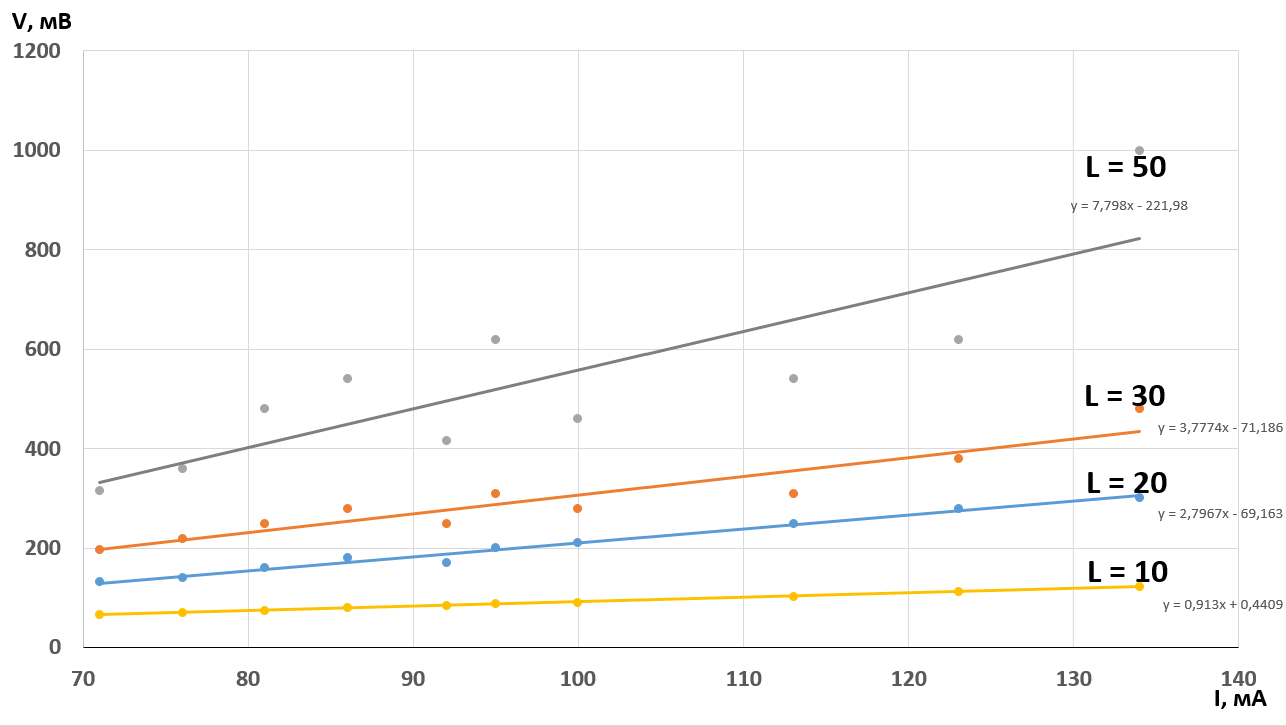
\includegraphics[width=\textwidth]{R}
    \end{figure}
    
    Из графика видно, что тангенс угла наклона и есть сопротивление: $R_{10} = 0.913, R_{20} = 2.797, R_{30} = 3.777, R_{50} = 7.798$.\\
    
    Давайте занулим коэффициент b, получим следующий график: 
    \begin{figure}[H]
        \centering
        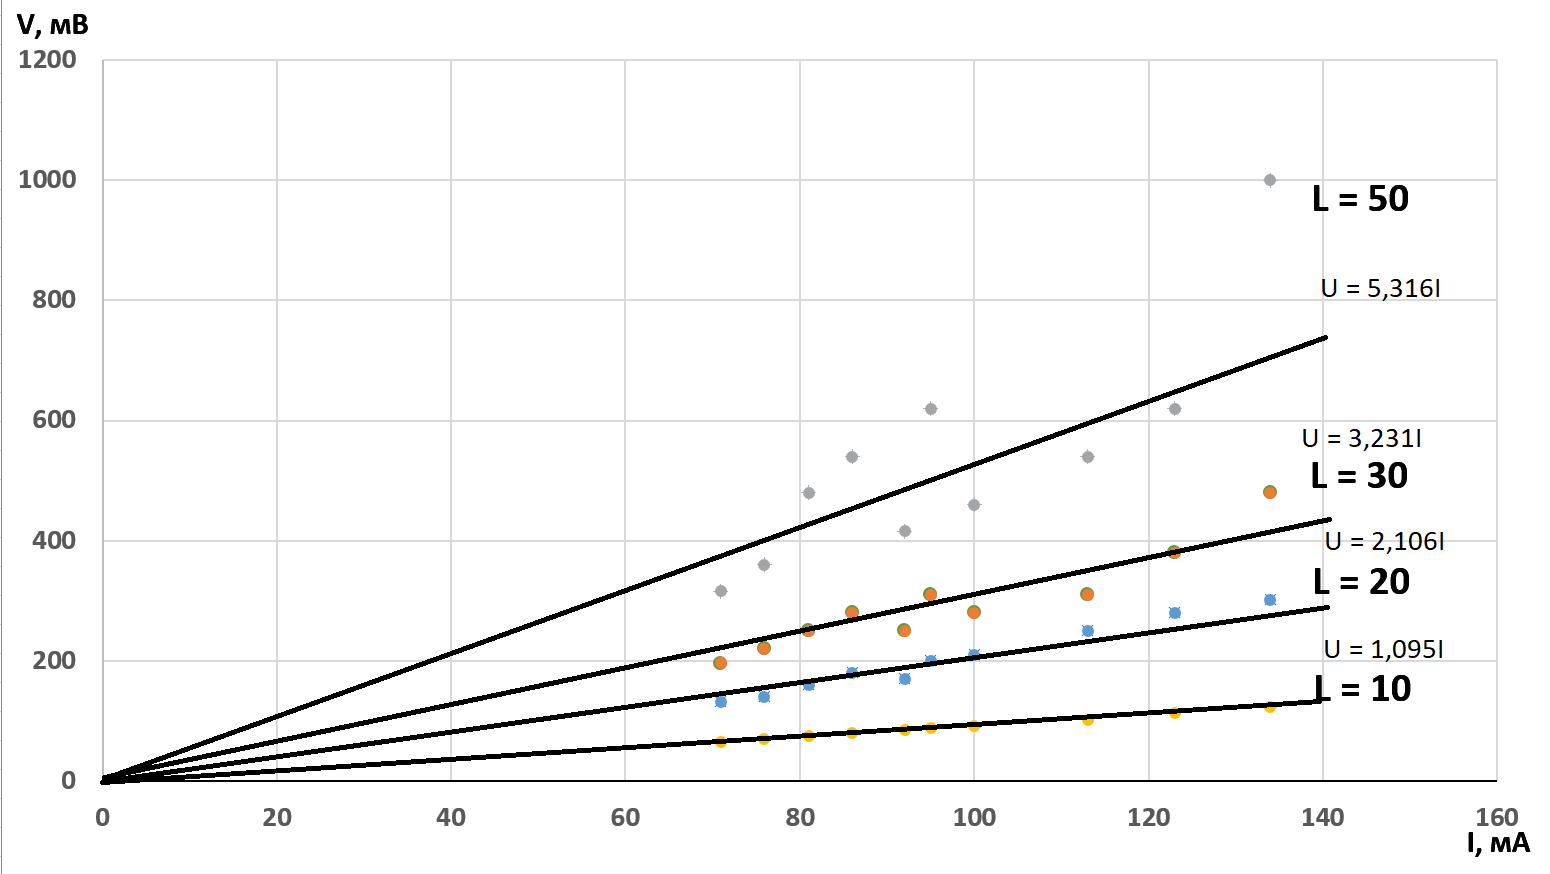
\includegraphics[width=\textwidth]{R_0}
    \end{figure}
    
    Давайте посчитаем среднее сопротивление по формуле:
    \begin{equation}
        R_{ср} = \frac{\sum_i R_i}{n}
    \end{equation}
    
    \[
        R_{ср_{10}} = 1.0949;
        R_{ср_{20}} = 2.1067;
        R_{ср_{30}} = 3.2282;
        R_{ср_{50}} = 5.3200.
    \]
    
    Найдем среднюю погрешность для l = 10 см, 20 см, 30 см, 50 см, пользуясь следующей формулой:
    \begin{equation}
        \sigma_{ср} = \frac {\sqrt{\sum_{i}^{n}(R_i - R_{ср})^2}} {n}
    \end{equation}
    
    \[
        \sigma_{ср_{10}} = 0.0019;
        \sigma_{ср_{20}} = 0.0073;
        \sigma_{ср_{30}} = 0.0126;
        \sigma_{ср_{50}} = 0.0157.
    \]
    
    Давайте найдем удельно сопротивление по формуле (1) и погрешность по следующей формуле:
    \begin{equation}
        \frac {\sigma_p}{\rho} = \sqrt {(\frac{\sigma R}{R})^2 + (2\frac{\sigma d}{d})^2 + (\frac{\sigma l}{l})^2}
    \end{equation}
    
    \begin{table}[H]
        \centering
        \begin{tabular}{|c|c|c|}
        \hline
        L, см & $\rho, 10^{-4}$ Ом$\dot$см & $\sigma_{\rho}, 10^{-6}$ Ом$\dot$см \\ \hline
        10 & 1.03 & 6\\ \hline
        20 & 1.06 & 6\\ \hline
        30 & 1.05 & 6\\ \hline
        50 & 1.02 & 6\\ \hline
        \end{tabular}
    \end{table}

\section {Обсуждение результатов} 
    Значения удельного сопротивления нихрома совпадают с табличными. $R_{ср}$ отличаются от наиболее точного измерения (с помощью моста Уинстона) по многим факторам: 
    \begin{enumerate}
        \item Неточностью программного вычисления
        \item Взятие бесконечно большого сопротивления у вольтметра 
        \item Округлением значений напряжения и тока при измерениях 
    \end{enumerate}

    При обнулении коэффициента b, мы получаем значения сопротивления наиболее приближенные к физическим законам, нежели чем при построении прямой с помощью метода наименьших квадратов.  

\section {Заключение}
    Проведя множество измерений, пользуясь электрической схемой, мы вычислили сопротивления проволоки определенной длины (10 см, 20 см, 30 см, 50 см), максимально приближенные к точному, вычисленными с помощью моста Уинстона.   

\end{document}
